\chapter{Genauer Vergleich}

In diesem Kapitel werden die vorher ausgewählten Suchmaschinen genauer verglichen. Dafür werden alle vier Suchmaschinen aufgesetzt und getestet. Dabei wird Wert auf alle Aspekte gesetzt. Wie leicht lässt sich die Suchmaschine aufsetzen? Wie ist, falls vorhanden, das Webinterface? Wie funktionieren die Query’s und vor Allem wie viel Zeit benötigen diese? Da ich dieses Projekt nicht nach dieser Bachelor-Arbeit wohl nicht weiter verfolgen kann, ist es auch wichtig zu schauen, wie leicht ein neuer Administrator sich in das System einlernen kann, beziehungsweise wie leicht das System zu verstehen und administrieren ist. Deshalb wird auch die Dokumentation verglichen und geschaut, wie groß die Community der einzelnen Suchmaschinen ist. 

\section{Aufbau der Tests}

\subsection{Installation}

Im ersten Schritt wird die Installation bewertet, dabei wird geschaut, wie einfach es ist die Software zu installieren. Hierbei ist es wichtig zu schauen, wir simple die Installation ist. Existiert zum Beispiel ein Installations-Wizard? Wie ist die Konfiguration um das System zum Laufen zu kriegen? Wie viel muss manuell in den Dateien geändert werden?

\subsection{Oberfläche}

Als Nächstes folgt der Ersteindruck der Software und des Interfaces. Dabei wird geschaut, wie übersichtlich die Oberfläche ist, falls eine gegeben ist, und wie verständlich das System für Einsteiger ist. Dafür wird im ersten Schritt möglichst auf die Dokumentation verzichtet, um einen Ersteindruck zu liefern, wie gut die Oberfläche für sich selbst spricht. Dies dient dafür um, zu schauen wie der neue Administrator sich ohne Vorkenntnisse einarbeiten kann. Besondere Punkte dabei sind zum Beispiel: Wie viel kann man über die Oberfläche konfigurieren? Lassen sich Updates direkt über die Oberfläche einspielen? Ist die Seite responsive? Wie funktioniert die Nutzerverwaltung?

\subsection{Dokumentation}

Im dritten Schritt wird die Dokumentation analysiert. Hierbei wird das Augenmerk auf die Übersichtlichkeit und Verständlichkeit gelegt. Es wird auch Wert darauf gelegt, inwiefern die Dokumentation ohne Fachkenntnisse zu verfolgen ist. Da in diesen Kurztest nicht alle Funktionen durchgetestet werden können, ist es leider auch nicht möglich zu schauen, ob alle Funktionen korrekt und ausführlich dokumentiert sind. Sollte allerdings schon von den Grundfunktionen eine schlechte oder fehlende Dokumentation auffallen wird dies natürlich erwähnt. 

\subsection{Datenschutz}

Hier geht es darum zu schauen, ob das Tool nach Hause telefoniert. Dann soll noch überprüft werden, ob die Logdateien anonymisiert und nach gewisser Zeit gelöscht werden können.

\subsection{Absetzen einer Anfrage und Integration in PHP}

Im letzten Schritt werden einige Query’s abgesetzt. Dies wird zum einen über ein die Oberfläche geschehen, falls vorhanden, und was wichtiger ist über die Schnittstelle für PHP. Dafür wird ein PHP-Script geschrieben und die Laufzeit des Scripts gemessen.

Der erste Query ist der am Aktuell am längsten laufende Query vom Dietrich-Online Projekt. Dabei werden alle Lemmata vom Buchstaben S angezeigt.


Als werden diverse Query’s für die Fehlerliste abgearbeitet. Die Fehlerliste eignet sich deshalb besonders gut für solche Query’s, da die 3 Tabellen umfasst, allerdings keine Verbindung zum restlichen Projekt besitzt. \ref{img:errorListStructure}

\begin{figure}
	\centering
	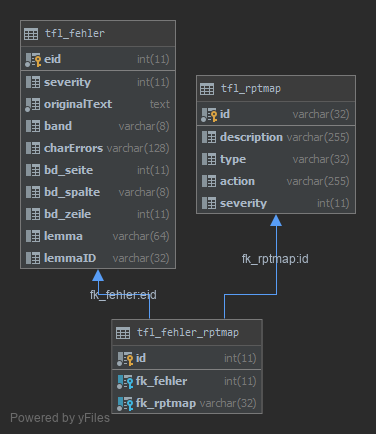
\includegraphics[width=0.5\linewidth]{images/structure_errormodule.png}
	\caption{Tabellenaufbau der Fehler Liste}
	\label{img:errorListStructure}
\end{figure}

Im ersten Query werden die Fehlercodes zu den einzelnen Fehlern direkt an die Tabelle angebunden. 

\lstset{language=SQL}
\begin{lstlisting}[frame=single]  % Start your code-block

SELECT  fehler.eid,
        fehler.originalText,
        fehler.band,
        fehler.bd_seite,
        fehler.bd_spalte,
        fehler.bd_zeile,
        fehler.lemma,
        fehler.charErrors,
        fehlercodes.description
FROM tfl_fehler fehler

LEFT JOIN tfl_fehler_rptmap fehler_fehlercode_map 
ON fehler.eid = fehler_fehlercode_map.fk_fehler

LEFT JOIN tfl_rptmap fehlercodes 
ON fehlercodes.id = fehler_fehlercode_map.fk_rptmap

WHERE fehler.band = ('1')
AND fehler.severity > 3
ORDER BY fehler.eid;
\end{lstlisting}


Da es für jeden Eintrag mehrere Fehler geben kann und diese Fehler für jeden Eintrag verfügbar sind, gibt es hier eine n zu m Beziehung. Um diese Abzubilden wurde die Tabelle tfl\_fehler\_rptmap eingefügt. Diese verbindet jeweils die ID’s mit den dazugehörigen Fehlercodes. 